	\section{Speed Reference Output Channel}\label{sec:speed-reference-output-channel}

	\subsection{Speed Control}\label{ssec:speed-control}
		\par
		For the braketests, somethings as important as measuring the speed of the rotor is controlling it, as mentioned in Subsection \ref{ssec:lowerLayerlHardware}. The rotor speed can be controlled in two ways:
			\begin{itemize}
				\item First way is the deceleration of the rotor with the aid of the brake system using the brake pads.
				\item Second way of controlling it by accelerating the rotor with the aid of the electric motor.
			\end{itemize}
		The electric motor used is a alternate current three-phase type, it in order to control it's speed a frequency inverter was used. The frequency inverter has many different controlling interfaces that lead to manipulating the three-phase electric system in order to control the engine's rotationary speed.
		\par
		In this project the frequency inverter used was the \textit{Weg CFW-08} (shown in Figure \ref{fig:wegCFW08}, according to \cite{wegCFW08Manual} there are many port interfaces that can be used to control the desired speed remotely. One of this ways is using one of the device's 0-10V analog input with 8-bit resolution. According to the datasheet, this analog input can be used as a speed reference with programmable gain (0-20), the input parameters are the lower limit speed (when the input is on 0V) and the upper limit speed (when the input is at 10V).

		\begin{figure}[htbp]
			\centering
				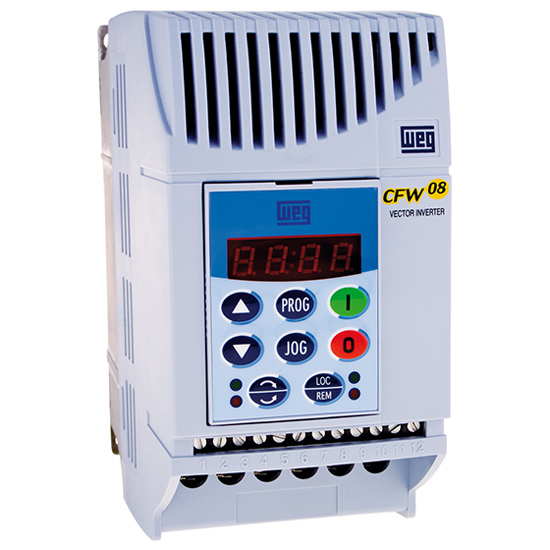
\includegraphics[scale=0.4]{figuras/fig-wegCFW08}
			\caption{Weg CFW-08 Frequency Inverter \cite{fig-wegCFW08}}
			\label{fig:wegCFW08}
		\end{figure}

		The issue is that this project is microcontrolled, and MCU's do not have analog outputs, so a DAC circuit will need to be implemented. The MCU output will be a PWM signal, moreover as mentioned in Section \ref{ssec:pwm}, a PWM signal can encode information on a pulse train signal and this information can be decoded using a LPF, \textit{i.e.} performing a digital to analog conversion.

	\subsection{Filter characteristics definition}\label{ssec:filterCharacteristicsDefinition}
		\par
		Fortunately the microcontroller has pre-configured PWM \textit{(Pulse Width Modulation)}, a PWM signal can encode a analog voltage value proportional to it`s duty cycle, and this is usually done with the aid of a low pass filter that will extract this analog voltage from the PWM signal. As said in the previous paragraph the frequency inverter used in this project is the \textit{Weg CFW-08}, and it's analog input has a zero to ten voltage input with eight bits of resolution. We can calculate the minimal voltage difference that will change the output frequency of the device using Equation \ref{eqn:minVoltage}, in which $\Delta V$ is the minimal voltage difference, $V_{max}$ is the maximum voltage and \textit{"n"} is the number of bits of the input resolution.

			\begin{equation}\label{eqn:minVoltage}
				\Delta V=\frac{V_{max}}{2^{n}}
			\end{equation}
	
		As mentioned in Section \ref{sec:mcu-hw}, the choosen MCU has a five volts high logic level, this voltage level will need amplification in order to best suit the zero to ten volts input from the frequency inverter. However, as alrealdy mentioned in Section \ref{ssec:speed-control} the analog input of the frequency inverter already has a 0-20 programmable gain that will be set to two. 
		\par
		The maximum ripple is the $\Delta V$ from Equation \ref{eqn:minVoltage}. Equation \ref{eqn:atte} \cite{metivier2013pwm} gives the necessary $\frac{dB}{decade}$ attenuation to guarantee a PWM converted signal desired ripple.

	 		\begin{equation}\label{eqn:atte}
				A_{dB}=20\cdot log \left( \frac{V_{RIPPLE}}{V_PWM} \right) 
			\end{equation}
			
		As the $V_{PWM}$ will already be aplified prior to filtering, $V_{PWM}=V_{max}$, this will produce the following Equation \ref{eqn:attenuation}.
		
			\begin{equation}\label{eqn:attenuation}
				A_{dB}=-20 \cdot n \cdot log \left( 2 \right) 
			\end{equation}
	
		And Equation \ref{eqn:LPFcuttoffFrequency} \cite{metivier2013pwm}, is used to calculate the maximum needed cuttoff frequency for the further to be designed LPF (\textit{Low-Pass-Filter}) in order to convert the PWM signal to a analog voltage. The slope value is the filter slope and for first order filters and second order filters this slope value is equal respectively to 20dB/decade and 40dB/decade \cite{metivier2013pwm}.
	
			\begin{equation}\label{eqn:LPFcuttoffFrequency}
				f_{c}=f_{PWM} \cdot 10^{-\frac{A_{dB}}{Slope}}
			\end{equation}

		It is possible to combine all this equations into one single equation to calculate the needed cutoff frequency, is this done in Equation \ref{eqn:LPFcuttoffFrequency2}.

			\begin{equation}\label{eqn:LPFcuttoffFrequency2}
				\begin{split}
					f_{c}=f_{PWM} \cdot 10^{-\frac{A_{dB}}{Slope}}	\\
					f_{c}=f_{PWM} \cdot 10^{-\frac{-20 \cdot n \cdot log \left( 2 \right)}{Slope}}	\\
					f_{c}=f_{PWM} \cdot 10^{log \left( 2^{\frac{20 \cdot n }{Slope}} \right)}	\\
					Knowing:	\\
					x \cdot log \left( A \right) =  log \left( A^{X} \right) \\
					10^{log \left( A \right) } = A	\\
					So:	\\
					f_{c}=f_{PWM} \cdot  2^{\frac{20 \cdot n}{Slope}}
				\end{split}
			\end{equation}

	
		As shown in Appendix \ref{app:microCode}, the default PWM frequency for the defined pins are $f_{PWM}=490Hz$, also $n=8$ (number of bits of the ADC from the frequency inverter) and as according to \cite{metivier2013pwm}, a second order LPF is better for converting a PWM signal to voltage and it has by default $Slope=-40dB/decade$, using Equation \ref{eqn:LPFcuttoffFrequency2} it is possible to calculate a maximum cutoff frequency of 30.625Hz. 

	\subsection{Sallen-Key Low Pass Active Filter}\label{ssec:sallen-key-low-pass-active-filter}
	
		The Sallen-Key LPF setup is probably one of the best second order filters architectures available \cite{dorfsvodoba2014}, this setup is displayed on Figure \ref{fig:sallenKeyLPF}.

		\begin{figure}[htbp]
			\centering
				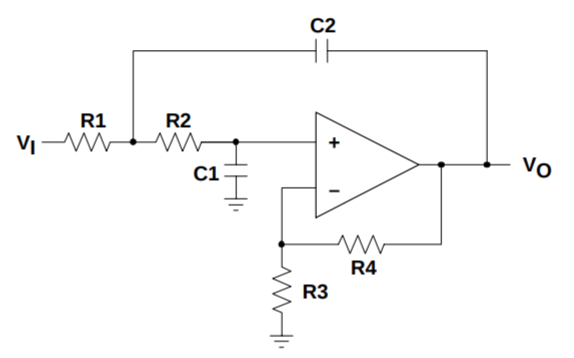
\includegraphics[scale=0.6]{figuras/fig-sallenKeyLPF}
			\caption{Sallen-Key Active Low Pass Filter \cite{texas1999sallenkey}}
			\label{fig:sallenKeyLPF}
		\end{figure}

		According to \cite{texas1999sallenkey}, this filter setup has a cutoff frequency defined by Equation \ref{eqn:sallenKeyTransferFunction}.

		\begin{equation}\label{eqn:sallenKeyCutoffFrequency}
			f_{c}=\frac{1}{2 \cdot \pi \sqrt{R_{1} \cdot R_{2} \cdot C_{1} \cdot C_{2}}} 
		\end{equation}

		Using values of R1=100k$\Omega$, R2=100k$\Omega$, C1=100nF and C2=100nF means having a cutoff frequency of 15.91Hz

		\subsection{Complete Circuit}\label{ssec:pwm-to-speed-reference-circuit}
	
		Based on all the previously calculations and on \cite{texas1999sallenkey}, the final circuit will be the one in Figure \ref{fig:pwmToSpeedReferenceCircuit}. Besides the main components of the filter the added components were two bypass capacitors (C1 and C4), TZ1 is a TVS used to protect the circuit from any transient voltage coming from the cable. Moreover, R1 was added to limit the current that is drained from the analog output. The port \textit{AOU$\_$1} is a feedback that goes to a analog input of the MCU so the output voltage can be adjusted by varying the duty cycle.

	
		\begin{figure}[htbp]
			\centering
				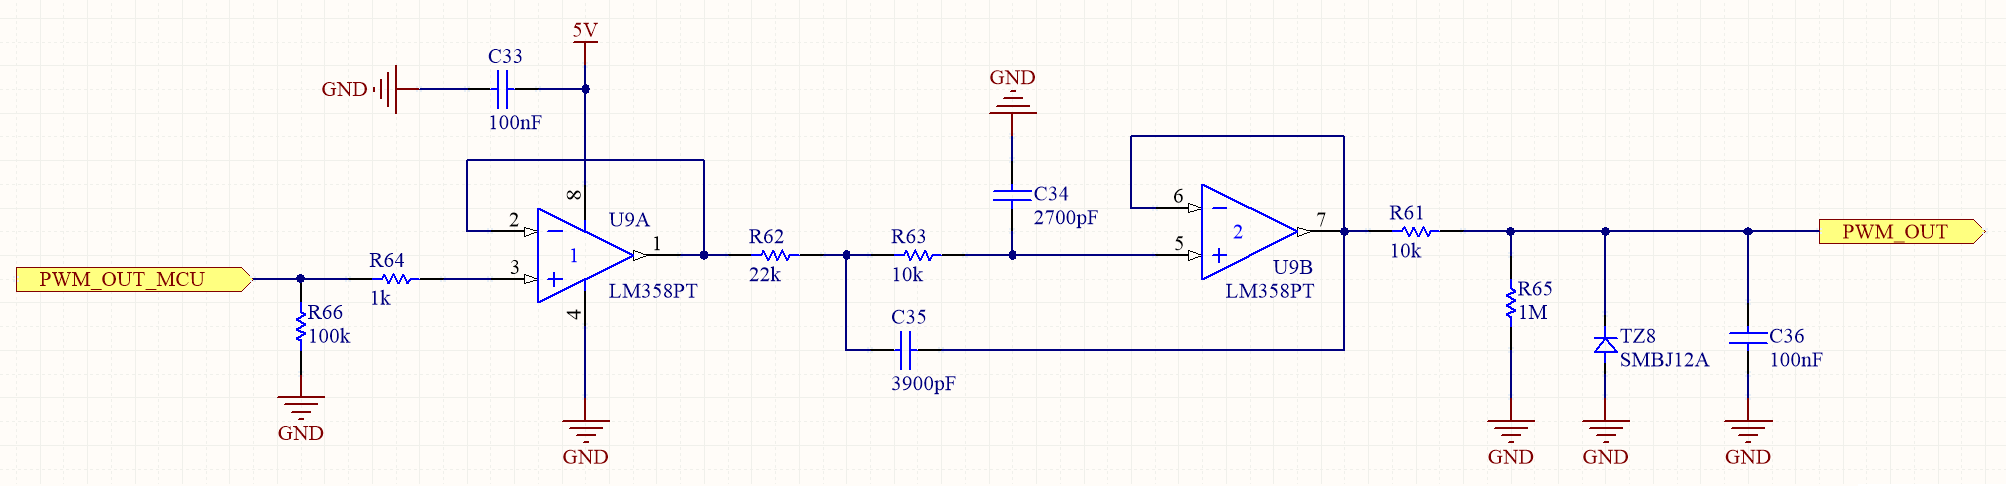
\includegraphics[scale=0.6]{figuras/fig-pwmToSpeedReferenceCircuit}
			\caption{PWM to Speed Reference Circuit}
			\label{fig:pwmToSpeedReferenceCircuit}
		\end{figure}

		Although only one analog output is needed, another one will be placed on the PCB in order to allow the circuit to be used on other appliances on possible future projects.